\chapter{Анализ предметной области}

В данном разделе вводятся основные определения и описываются важность и актуальность задачи упрощения текстов.

\section{Задача упрощения текстов}


Существуют различные формулировки задачи упрощения текста. 
Так, в статье \cite{siddharthan_survey_2014} даются определения в двух смыслах:
\begin{itemize}
	\item упрощение текста в узком смысле - это процесс уменьшения его лингвистической сложности при сохранении исходной информации и смысла;
	\item в более широком смысле упрощение текста охватывает и другие операции: смысловое изменение для упрощения как формы, так и содержания; краткое изложение текста для исключения второстепенной или избыточной информации.
\end{itemize}

В статье \cite{martin_muss_2021} упрощением предложений называют процесс, целью которого является получение более легкого для чтения и понимания текста за счет уменьшения его лексической и структурной сложности.

При этом задача упрощения текстов относится к области NLP (Natural language processing, обработка текстов на естественном языке) и имеет много общего с другими задачами из этой сферы - машинным переводом, перефразированием и обобщением (резюмированием) текста\cite{zhu_monolingual_2010}. 

Важно отметить отличие упрощения текста от его обобщения, так как эти задачи зачастую путают. Отличие заключается в том, что во втором случае основное внимание уделяется сокращению длины исходных данных и удалению из них второстепенной информации. И хотя обобщенные тексты, как правило, короче, это не всегда так, и обобщение может привести к увеличению длины полученных предложений\cite{shardlow_survey_2014}, что сделает текст более сложным для чтения. В рамках же упрощения текста обычно сохраняется все содержание, а основной целью считается сделать его более легким для восприятия.

\section{Актуальность}
В последние десятилетия количество неструктурированных текстовых данных резко возросло в связи с развитием Интернета. Как следствие, возросла и потребность в их упрощении, что показано на рисунке \ref{fig:growth_of_interest}. 


%\clearpage

\begin{figure}[h!]
	\begin{center}
		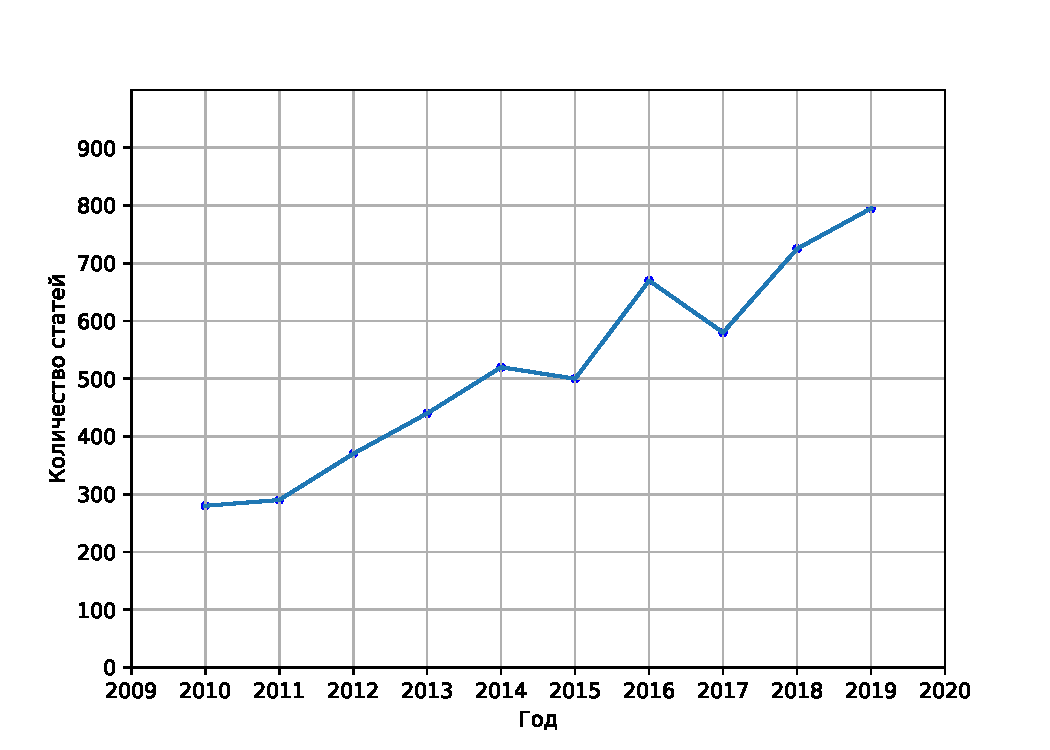
\includegraphics[pages=-, scale=0.9]{./inc/img/graph.pdf}
		\caption{График роста интереса к теме упрощения текста. Создано на основе статистики Google Scholar по поисковым запросам <<Text Simplificatio>> (упрощениие текстов),  <<Lexical Simplification>> (лексическое упрощение), <<Syntactic Simplification>> (синтаксическое упрощение)\cite{sikka_survey_2020}}  
		\label{fig:growth_of_interest}
	\end{center}
\end{figure}

%\begin{figure}[h!]
	
%	\centering{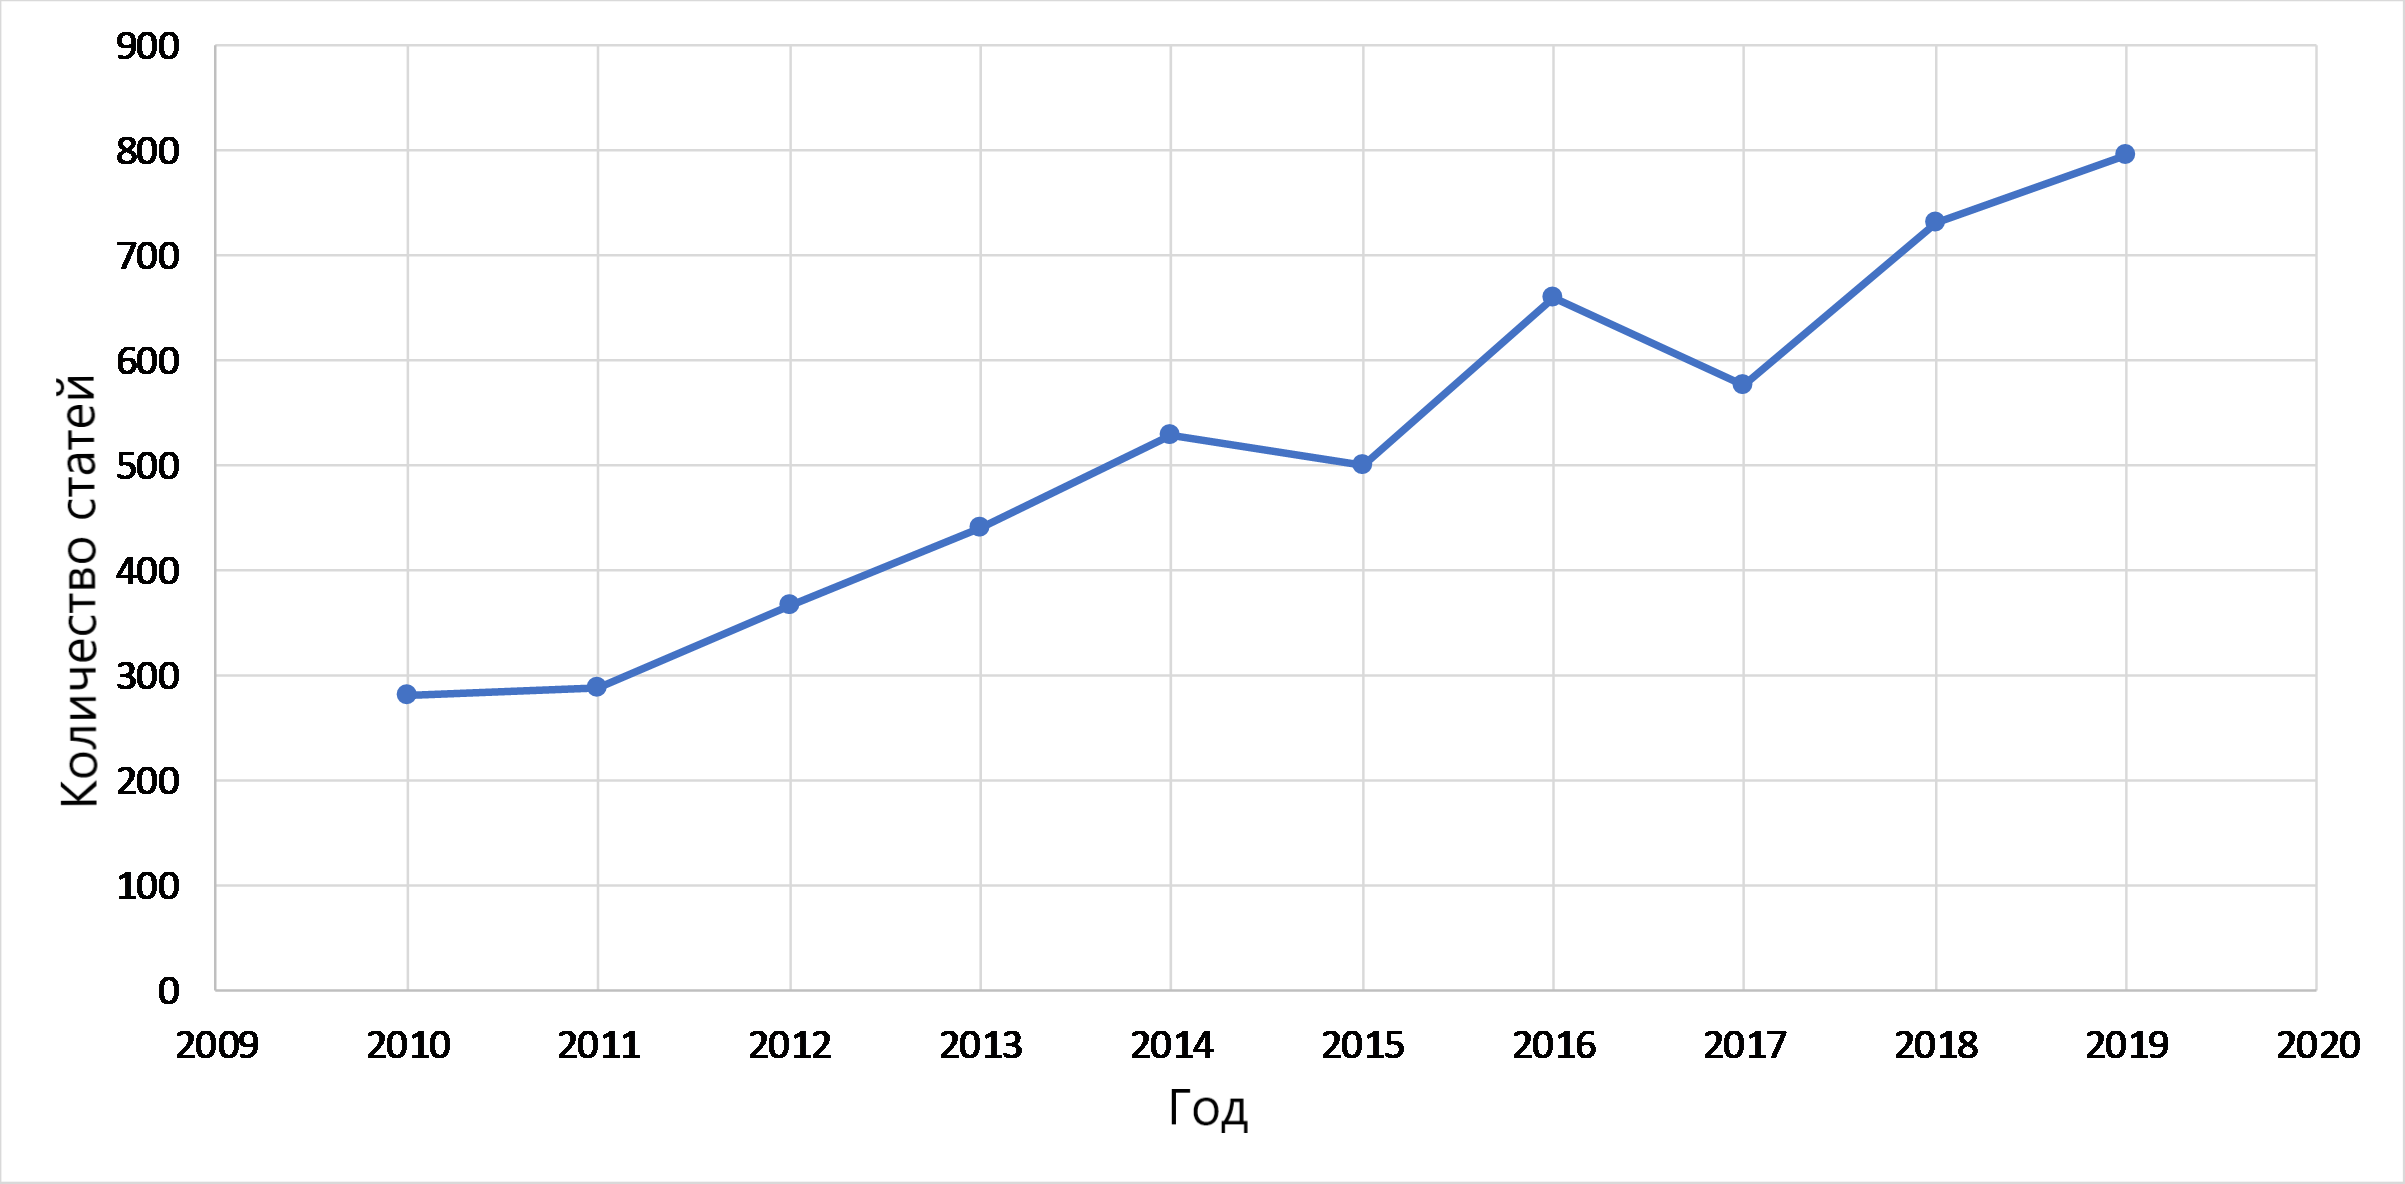
\includegraphics[scale=0.25]{inc/img/growth_of_interest.png}}
	
%	\caption{График роста интереса к теме упрощения текста. Создано на основе статистики Google Scholar по поисковым запросам "Text Simplification" ("Упрощениие текстов"),  "Lexical Simplification" ("Лексическое упрощение"), "Syntactic Simplification" ("Синтаксическое упрощение")\cite{sikka_survey_2020}}
	
%	\label{fig:growth_of_interest}
	
%\end{figure}

Упрощение текстов необходимо для различных задач и целевых аудиторий: 
\begin{itemize}
	\item в качестве этапа подготовки текста перед его обобщением ~\cite{finegan_dollak_sentence_2016}; 
	\item для людей, изучающих иностранный язык, и детей, учащихся читать (требуется лексическое упрощение для сокращения количества специализированных и нечастотных слов) ~\cite{liu_simplification_2016};
	\item для людей с дислексией и афазией, для которых длинные слова и предложения могут представлять трудности;
	\item для людей, страдающих аутизмом (необходимо уменьшать количество образных выражений и синтаксическую сложность) ~\cite{evans_evaluation_2014}.
\end{itemize}

\section{Данные}
%\textbf{\textit{проблема и круг вопросов, необходимых для ее решения}}\\

Упрощение предложений привлекло многих исследователей в связи с появлением больших параллельных корпусов. Наиболее известные из них составлены из английских текстов, например, PWKP и Wiki-large. Последний представляет собой большой параллельный корпус на английском языке, состоящий из сложных предложений, взятых из Википедии, и их выровненных упрощенных версий.

Подобных данных на других языках значительно меньше. Большой корпус на русском языке был собран, когда задача упрощения текстов была предложена в рамках международной конференции по компьютерной лингвистике и интеллектуальным технологиям DIALOGUE 2021\footnote{\url{http://www.dialog-21.ru/dialogue2021/results/}}. Организаторы подготовили обучающие и тестовые наборы на русском языке с использованием краудсорсинговой платформы, а также перевели тексты из Википедии (корпус RuWikiSimple). Другим источником данных могут стать результаты перевода, выполненные при помощи перефразирования\cite{kazan_federal_university}.  

Основная проблема в упомянутых данных заключается в том, что имеет место фокусировка на текстах Википедии. Это ограничивает исследования и приводит к неадекватности моделей на других типах данных ~\cite{kazan_federal_university}. 



\section*{Выводы из анализа предметной области}

Таким образом, акутальность задачи упрощения тексов в последнее десятилетие увеличивается, формируются новые корпуса на различных языках для обучения моделей.  При этом поставленная задача схожа с другими задачами из сферы NLP, а если использовать ее более широкое понятие, то она будет трудно отличима от задачи обобщения. Поэтому, чтобы разграничить эти два понятия, в данной работе будет рассматриваться задача упрощения предложений в более узком смысле, формулировка которой приведена выше (из статьи \cite{martin_muss_2021}).
